\documentclass[11pt]{amsart}
% Preamble of main.tex. Load after the document class.
\usepackage{amsmath,amssymb,amsthm,mathtools}
\usepackage[margin=1.1in]{geometry}
\setlength{\emergencystretch}{1em}
\usepackage{booktabs}
\usepackage[hidelinks]{hyperref}
\usepackage{enumitem}

\newtheorem{theorem}{Theorem}[section]
\newtheorem{proposition}[theorem]{Proposition}
\newtheorem{lemma}[theorem]{Lemma}
\newtheorem{corollary}[theorem]{Corollary}
\newtheorem{maintheorem}{Theorem}
\renewcommand{\themaintheorem}{\Alph{maintheorem}}
\theoremstyle{definition}
\newtheorem{definition}[theorem]{Definition}
\theoremstyle{remark}
\newtheorem{remark}[theorem]{Remark}

\newcommand{\R}{\mathbb{R}}
\newcommand{\C}{\mathbb{C}}
\newcommand{\Z}{\mathbb{Z}}
\newcommand{\Q}{\mathbb{Q}}
\newcommand{\T}{\mathbb{T}}
\newcommand{\CP}{\mathbb{CP}}
\newcommand{\eps}{\varepsilon}
\newcommand{\Cfg}{\mathcal{C}}
\newcommand{\Lw}{\mathcal{L}}
\newcommand{\Up}{\mathcal{U}}
\newcommand{\Dt}{\mathsf{D}}
\DeclareMathOperator{\vol}{vol}
\DeclareMathOperator{\dist}{dist}
\DeclareMathOperator{\area}{area}
\usepackage{tikz}

\hypersetup{
  pdftitle={Elementary packings of the four-ball and their limits},
  pdfauthor={Liang Song},
  pdfsubject={Symplectic ball packings},
  pdfkeywords={symplectic geometry, ball packing, toric domains, packing obstructions},
  pdflang={en-US}
}

\title{Elementary packings of the four-ball and their limits}
\author{Liang Song}
\email{sl12160010@gmail.com}
\date{}

\begin{document}
\begin{abstract}
We study symplectic packings of the four-ball by equal balls that are assembled from Traynor's toric trick and
from equivariant ``windows'' in the reduced spaces of the circle $(z_1,z_2)\mapsto(e^{it}z_1,e^{-it}z_2)$. On the
positive side, $n(n+1)$ balls fill the fraction $1-1/(2n+1)^2$ of a ball for every $n\ge2$, every $k\ge3$ balls fill
at least $1-1/\sqrt k$, and ten balls fill $360/361$. On the negative side we prove three obstructions for these
constructions at fixed $k$: a tensor-valued area invariant shows that lattice bookkeeping, even with different
circles on different polygonal pieces, can be exact only when $k$ is a square; a periodisation argument shows
that every packing whose profiles are balanced needs $A^2-\dist(A,\Z)^2\ge k$ for the capacity $A$ of the
target, which reproduces the sharp McDuff--Polterovich values for $k=6,7,8$; and eight full-height single-ball
columns need capacity at least $19/6$. The $n(n+1)$-ball and ten-ball configurations attain the balanced bound, so they are optimal among balanced
packings, and $360/361$ is also optimal among packings with eight full-height columns. For fixed non-square $k$,
density tending to $1$ by these methods would therefore need configurations that are neither lattice nor balanced; whether such configurations exist is open.
\end{abstract}
\maketitle

% =====================================================================================================
\section{Introduction}\label{sec:intro}

Let $B(a)\subset\C^2$ denote the open ball of capacity $a$ (unlike \cite{SongP1}, $B(a)$ is open here), so that the unit ball has capacity $\pi$. Gromov's
two-ball theorem \cite{Gromov1985} and the work of McDuff and Polterovich \cite{McDuffPolterovich1994} determine
the largest fraction $p_k$ of $B(1)$ that $k$ equal balls can fill for $k\le8$, and $p_9=1$ \cite{McDuffPolterovich1994};
Biran \cite{Biran1997} proved $p_k=1$ for all $k\ge9$, and his stability theorem \cite{Biran1999} explains the phenomenon in general. These proofs
pass through blow-ups, inflation and $J$-holomorphic curves and do not produce the embeddings. Explicit maximal
packings are known for $k\le6$ and for squares $k=d^2$ (Traynor \cite{Traynor1995}), for $k=7,8$ (Wieck's
symplectic tunnelling \cite{Wieck2009}; see also \cite{Opshtein2011}); folding and wrapping give further explicit packings
\cite{SchlenkHand,SchlenkBook,Schlenk2018}. For every $k\ge10$ and every $\eps>0$ an explicit Hamiltonian packing of
density $1-\eps$ is constructed in \cite{SongP1}, developing the twisted disc-bundle mechanism of
\cite{OpenAI2026}; it uses a non-toric disc-bundle model.

This paper treats the elementary side. The building blocks are Traynor's lemma, which puts a ball of capacity
$\lambda<1$ into the product of a unimodular triangle with a torus, and the circle
$S=\{(e^{2\pi it}z_1,e^{-2\pi it}z_2)\}$, whose reduced spaces are discs. Toric packings put the reduced slices of all
balls concentrically around the centre of each disc; windows allow some of them to sit off centre. The
bookkeeping is one-dimensional: each ball contributes a \emph{profile}, the area of its reduced slice as a
function of the moment $s=\pi|z_1|^2-\pi|z_2|^2$, and the profiles must fit under the profile
$c_A(s)=\frac12(A-|s|)$ of $B(A)$ (Figure~\ref{fig:ten}). The loss is visible as the part of $c_A$ that the
profiles leave uncovered.

\emph{Constructions.} Section~\ref{sec:setup} makes the class precise and proves a realisation theorem
(Theorem~\ref{thm:realise}) that turns a one-dimensional configuration into a symplectic embedding. In
Section~\ref{sec:families} we prove:
\begin{itemize}[leftmargin=2em]
\item \textbf{Theorem~\ref{thm:family}.} For every $n\ge2$, $n(n+1)$ balls of capacity $1$ fit into
  $B(n+\frac12)$: density $1-1/(2n+1)^2$.
\item \textbf{Corollary~\ref{cor:allk}.} For every $k\ge3$, $k$ balls of capacity $1$ fit into a ball with density
  at least $1-1/\sqrt k$.
\item \textbf{Proposition~\ref{prop:ten}.} Ten balls of capacity $1$ fit into $B(\frac{19}{6})$: density
  $\frac{360}{361}$.
\end{itemize}
Here ``fit'' means that for every $\lambda<1$ there is a symplectic embedding of the balls of capacity $\lambda$;
equivalently, closed balls of capacity $1$ embed into $B(A')$ for every $A'>A$.

\emph{Obstructions.} Section~\ref{sec:obstructions} explains why such constructions stop short of density $1$ for
fixed non-square $k$:
\begin{itemize}[leftmargin=2em]
\item \textbf{Theorem~\ref{thm:tensor}} (tensor area). If the moment triangle $\Delta(A)$ of $B(A)$ is cut into polygons with edges in integer
  directions and on each piece the profile for some linear circle of its own is a sum of unit lattice profiles, then
  $A\in\Z$.
  Consequently lattice configurations of $k$ balls for a single linear circle have density at most a constant
  $\rho_k<1$ when $k$ is not a square (Corollary~\ref{cor:gap}).
\item \textbf{Theorem~\ref{thm:newton}} (Newton barrier). If the $1$-periodisations of the profiles (push-forwards of
  volume under $s$) of $k$ disjoint sets of volume $\frac12$ in $B(A)$ add up to a constant, then $A^2-\dist(A,\Z)^2\ge k$, that is
  $A\ge\frac12(m+k/m)$ for the integer $m$ with $m^2-m<k\le m^2+m$. For $k=6,7,8$ this equals the sharp value
  $\frac52,\frac83,\frac{17}{6}$ of McDuff--Polterovich. The bound is attained for $k=n(n+1)$ by
  Theorem~\ref{thm:family} and for $k=10$ by Proposition~\ref{prop:ten}.
\item \textbf{Theorem~\ref{thm:eight}.} Eight full-height column profiles (single balls carried by columns of
  height $1$, Section~\ref{sec:eight}) under $c_A$ force $A\ge\frac{19}{6}$.
  Proposition~\ref{prop:ten} attains this.
\end{itemize}

These statements separate what the elementary picture can do from what it cannot. For $k=10$ it reaches
$\frac{360}{361}$; the missing $\frac1{361}$ is a concentric ball, and the obstructions say that it cannot be
removed by rearranging lattice pieces, by any balanced arrangement, or by an arrangement in which eight balls
are full-height single columns. Filling it requires unbalanced arrangements, and we know no toric or window
mechanism that provides one. The non-toric construction of \cite{SongP1}, which develops the disc-bundle mechanism of
\cite{OpenAI2026} in dimension four, reaches density $1-\eps$ for every $\eps>0$.

% =====================================================================================================
\section{Set-up and realisation}\label{sec:setup}

\subsection{Conventions}
On $\C^2$ with $\omega_0=\sum_j dx_j\wedge dy_j$ we write $\mu_j=\pi|z_j|^2$ and $\theta_j=\arg z_j/2\pi\in\R/\Z$, so
$\omega_0=d\mu_1\wedge d\theta_1+d\mu_2\wedge d\theta_2$ where $z_1z_2\ne0$. The ball $B(a)=\{\mu_1+\mu_2<a\}$ has
capacity $a$ and volume $a^2/2$; we write $\vol$ for Lebesgue measure. The unit ball of the Euclidean metric is
$B(\pi)$; since density is invariant under dilation, $k$ balls of capacity $1$ in $B(A)$ have density $k/A^2$, and
in the radius normalisation of the Epoch problem \cite{Epoch} this is $k/R^4$ with $R^2=A$. Let $\Delta(A)$ be the
closed triangle with vertices $(0,0),(A,0),(0,A)$ and $\Delta^\circ$ the open triangle with vertices
$(0,0),(1,0),(0,1)$.

A \emph{unimodular triangle} is an open triangle $L(\Delta^\circ)+v$ with $L\in GL(2,\Z)$ and $v\in\R^2$; its
vertices lie in a translate $v+\Z^2$. A \emph{primitive-edge triangle} is an open triangle of area $\frac12$ one of whose
edge vectors is a primitive integer vector. Unimodular triangles are primitive-edge triangles. For an open set
$T\subset\R^2$ we call
\[
\ell_T(s)=\bigl|\{y:(s,y)\in T\}\bigr|
\]
its \emph{profile}; for a triangle of area $\frac12$ it is a tent of integral $\frac12$.

\begin{lemma}[Traynor]\label{lem:traynor}
Let $T$ be a primitive-edge triangle and $\lambda<1$. There is a symplectic embedding of $B(\lambda)$ into
$T\times\T^2\subset(\R^2\times\T^2,\,dp_1\wedge dq_1+dp_2\wedge dq_2)$, $\T^2=\R^2/\Z^2$, whose image has compact
closure in $T\times\T^2$.
\end{lemma}

\begin{proof}
Traynor \cite{Traynor1995} gives, for every $\lambda'<1$, a symplectic embedding $\tau$ of $B(\lambda')$ into
$\Delta^\circ\times(0,1)^2\subset\R^2\times\R^2$ (see also \cite[\S4.1, Lemma~4.2]{SchlenkHand}).
Take $\lambda<\lambda'<1$; then $\tau(\overline{B(\lambda)})$ is compact. Let $u$ be a primitive integer edge vector
of $T$ and $v$ its initial vertex, and let $L$ be the matrix with columns $u$ and the other edge vector at $v$;
then $|\det L|=2\area T=1$ and $T=L(\Delta^\circ)+v$. The map $(p,q)\mapsto(Lp+v,L^{-T}q)$ is linear symplectic. The
parallelogram $Q=L^{-T}(0,1)^2$ is spanned by $w_1=L^{-T}e_1$ and $w_2=L^{-T}e_2$; since $w_2\perp Le_1=u$ and
$\langle w_2,Le_2\rangle=1$, $w_2=\pm Ju$ with $J$ the rotation by a right angle, a primitive integer vector. A
parallelogram spanned by vectors $w_1,w_2$ with $|\det(w_1,w_2)|=1$ and $w_2$ primitive in $\Z^2$ injects into
$\R^2/\Z^2$: if $aw_1+bw_2\in\Z^2$ with $|a|,|b|<1$, then $\det(w_2,aw_1+bw_2)=\pm a\in\Z$, so $a=0$, and $bw_2\in\Z^2$
forces $b=0$. Composing gives the embedding.
\end{proof}

\subsection{The \texorpdfstring{$S$}{S}-chart}
Let $s=\mu_1-\mu_2$ and $\beta(s)=\max(0,-s)$. On $\{z_1\ne0\}$ define
\[
\Phi(z_1,z_2)=(s,\theta,w),\qquad \theta=\theta_1,\quad w=z_2\,z_1/|z_1|,
\]
with values in $F=\R\times(\R/\Z)\times\C$, $\omega_F=ds\wedge d\theta+d\,\mathrm{Re}\,w\wedge d\,\mathrm{Im}\,w$.
In polar coordinates $x=\pi|w|^2$, $\varphi=\arg w/2\pi$ we have $(s,x,\theta,\varphi)=(\mu_1-\mu_2,\mu_2,\theta_1,
\theta_1+\theta_2)$, an integral linear change of action-angle coordinates, so $\Phi^*\omega_F=\omega_0$. The map
$\Phi$ is an $S$-equivariant symplectomorphism onto $\{s+\pi|w|^2>0\}$ ($S$ acts by translation of $\theta$), with
inverse $z_1=\sqrt{(s+\pi|w|^2)/\pi}\,e^{2\pi i\theta}$, $z_2=we^{-2\pi i\theta}$, and
\begin{equation}\label{eq:ball-chart}
\Phi\bigl(B(A)\cap\{z_1\ne0\}\bigr)=\bigl\{(s,\theta,w):\ \beta(s)\le\pi|w|^2<\tfrac12(A-s),\ s+\pi|w|^2>0\bigr\}.
\end{equation}
The reduced space of $B(A)$ at level $s$ is a disc of area
\[
c_A(s)=\tfrac12(A-|s|)\qquad(|s|<A),
\]
with a cone point at $s=0$; in the chart it is the region \eqref{eq:ball-chart} with $s$ fixed, a disc centred at
$w=0$ for $s>0$ and an annulus around the hole $\{\pi|w|^2\le -s\}$ (the axis $z_1=0$) for $s<0$. Let
$\Omega_A=\{(s,x):\beta(s)<x<\frac12(A-s)\}$; it is the image of the interior of $\Delta(A)$ under
$(\mu_1,\mu_2)\mapsto(\mu_1-\mu_2,\mu_2)$, and $\ell_{\Omega_A}=c_A$.

\subsection{Configurations}
We use a second copy of $F$, with coordinates $(s,\theta,\zeta)$, as the model for windowed pieces, and write
$\nu=\pi|\zeta|^2$.

\begin{definition}\label{def:config}
A \emph{configuration in $B(A)$} consists of
\begin{enumerate}[label=(\roman*),leftmargin=2em]
\item finitely many pairwise disjoint primitive-edge triangles in $\Omega_A$ (the \emph{corner items}), divided into a
  lower family $\Lw$ and an upper family $\Up$;
\item finitely many \emph{columns} $\Cfg_1,\dots,\Cfg_J$, each a finite set of pairwise disjoint primitive-edge triangles
  in the half-plane $\{(s,\nu):\nu>0\}$ (the \emph{column items}),
\end{enumerate}
such that, with $\sup\emptyset=0$,
\begin{gather*}
u_j(s)=\sup\{\nu:(s,\nu)\in\textstyle\bigcup\Cfg_j\},\\
u^-(s)=\sup\bigl(\{\beta(s)\}\cup\{x:(s,x)\in\textstyle\bigcup\Lw\}\bigr),\qquad
u^+(s)=\inf\bigl(\{\tfrac12(A-s)\}\cup\{x:(s,x)\in\textstyle\bigcup\Up\}\bigr),
\end{gather*}
we have $u_j=0$ outside $(-A,A)$ and
\begin{equation}\label{eq:budget}
u_1(s)+\dots+u_J(s)\le\max\bigl(0,\,u^+(s)-u^-(s)\bigr)\qquad\text{for all }s.
\end{equation}
The \emph{items} are all these triangles; their number $k$ is the number of balls. The configuration is a
\emph{lattice configuration} if every item is a unimodular triangle. It is \emph{exact} if $k=A^2$.
\end{definition}

Corner items are toric: they are concentric annuli or discs in each reduced disc. Column items are toric in the
model copy of $F$; condition \eqref{eq:budget} says that the columns fit side by side into the band of the reduced
disc left free by the corner items. Since the items of a column are disjoint and lie below $u_j$, and the corner
items lie below $u^-$ or above $u^+$,
\begin{equation}\label{eq:bookkeeping}
\sum_{T}\ell_T\le c_A\quad\text{on }\R,\qquad\text{so}\qquad k=2\sum_T\int\ell_T\le A^2,
\end{equation}
with equality almost everywhere exactly when the configuration is exact. The functions $u_j$, $u^-$ and $-u^+$ are
lower semicontinuous, so \eqref{eq:budget} holds everywhere as soon as it holds almost everywhere.
Figure~\ref{fig:slice} shows a reduced slice.

\begin{figure}[t]
\begin{minipage}[c]{0.5\textwidth}
\centering
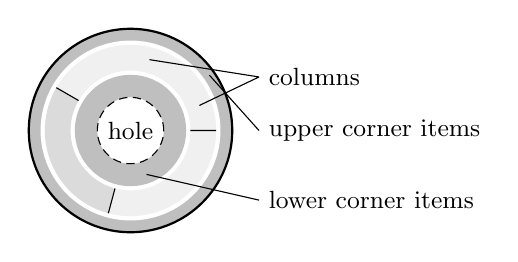
\begin{tikzpicture}[font=\small,scale=0.68]
  \fill[gray!50] (0,0) circle (1.9);
  \fill[white] (0,0) circle (1.68);
  \fill[gray!12] (0:1.12) arc (0:150:1.12)--(150:1.6) arc (150:0:1.6)--cycle;
  \fill[gray!28] (150:1.12) arc (150:255:1.12)--(255:1.6) arc (255:150:1.6)--cycle;
  \fill[gray!12] (255:1.12) arc (255:360:1.12)--(360:1.6) arc (360:255:1.6)--cycle;
  \draw (0:1.12)--(0:1.6) (150:1.12)--(150:1.6) (255:1.12)--(255:1.6);
  \fill[gray!50] (0,0) circle (1.04);
  \fill[white] (0,0) circle (0.62); \draw[densely dashed] (0,0) circle (0.62);
  \draw[thick] (0,0) circle (1.9);
  \node at (0,0) {hole};
  \draw (0.3,-0.82)--(2.4,-1.3) node[right]{lower corner items};
  \draw (75:1.37)--(2.4,1.0) (20:1.37)--(2.4,1.0) node[right]{columns};
  \draw (35:1.8)--(2.4,0.0) node[right]{upper corner items};
\end{tikzpicture}
\end{minipage}\hfill
\begin{minipage}[c]{0.47\textwidth}
\caption{A reduced slice of $B(A)$ at a level $s<0$ in the $S$-chart (schematic): the $w$-disc of area $c_A(s)$
with the hole $\pi|w|^2\le-s$ removed; for $s>0$ there is no hole. Corner items occupy concentric annuli (dark),
columns occupy angular sectors of the band between them (light); \eqref{eq:budget} says that the sectors fit.}
\label{fig:slice}
\end{minipage}
\end{figure}

\begin{theorem}[Realisation]\label{thm:realise}
Let a configuration in $B(A)$ with $k$ items be given and let $\lambda<1$. There is a symplectic embedding of $k$
disjoint copies of $B(\lambda)$ into $B(A)$. The copy assigned to a corner item $T$ lies in
$\Phi^{-1}\{(s,\theta,w):(s,\pi|w|^2)\in T\}$, and the copies assigned to a column $\Cfg_j$ lie in the image of an
$S$-equivariant symplectic embedding of an $S$-invariant neighbourhood of their model positions.
\end{theorem}

The embedding is given by explicit formulas built from Lemma~\ref{lem:traynor}, linear maps, the
area-preserving maps below (which involve square roots and an arcsine), a fixed mollifier, sup- and
inf-envelopes, and the quadrature \eqref{eq:G}. It is an embedding, not a Hamiltonian flow. By the connectedness of spaces of ball packings of $B^4$ \cite{McDuff1998}, applied to the open ball
viewed as $\CP^2\setminus\CP^1$, two packings of the same balls are isotopic through packings of a slightly larger
ball, so the embedding is the restriction of the time-one map of a compactly supported Hamiltonian on $\C^2$; we do
not make that Hamiltonian explicit.

\begin{proof}
\emph{Balls.} For each item $T$ Lemma~\ref{lem:traynor} gives an embedding of $B(\lambda)$ into $T\times\T^2$ with
image in a compact set $K_T$. For a corner item read $(p,q)=((s,x),(\theta,\varphi))$ and compose with $\Phi^{-1}$;
this embeds the ball into $B(A)$ because $T\subset\Omega_A$ and \eqref{eq:ball-chart} holds. Corner items are
disjoint, so these images are disjoint. For a column item read $(p,q)=((s,\nu),(\theta,\psi))$ with
$\zeta=\sqrt{\nu/\pi}\,e^{2\pi i\psi}$; this places the ball into the model $F$. Let $K^{(j)}$ be the union of the
$K_T$ over $T\in\Cfg_j$, $K^\Lw$ and $K^\Up$ the unions over lower and upper corner items, and denote by $\pi$
the projection to the $(s,\nu)$- or $(s,x)$-plane and by $S_j$ the projection of $K^{(j)}$ to the $s$-axis.

\emph{Margins.} The compact set $\pi(K_T)$ lies in the open triangle $T$. Fix $\eta>0$ such that the closed
$9\eta$-neighbourhood of $\pi(K_T)$ in the sup-norm lies in $T$ for every item, and put $M=8$. Then for all
$s,t$ with $|s-t|\le3\eta$: if $(t,\nu)\in\pi(K^{(j)})$ then $u_j(s)\ge\nu+M\eta$; if $(t,x)\in\pi(K^\Lw)$ then
$u^-(s)\ge x+M\eta$; if $(t,x)\in\pi(K^\Up)$ then $u^+(s)\le x-M\eta$. Write
$k_j^r(s)=\max\{\nu:(t,\nu)\in\pi(K^{(j)}),\,|t-s|\le r\}$ (and $0$ if there is no such point), so
$u_j(s)\ge k_j^{3\eta}(s)+M\eta$ whenever $\dist(s,S_j)\le3\eta$.

\emph{Smoothing.} Let $\rho$ be a smooth probability density supported in $[-\eta,\eta]$. For a bounded function
$g$ put $g^{\vee}(s)=\sup_{|t-s|\le\eta}g(t)$ and $g^{\wedge}(s)=\inf_{|t-s|\le\eta}g(t)$. If $g$ is upper
semicontinuous, so is $g^\vee$ (a supremum over a compact family), and if $g$ is lower semicontinuous, so is
$g^\wedge$; in these cases they are Borel, $g^\vee*\rho$ and $g^\wedge*\rho$ are smooth, and
\begin{equation}\label{eq:smooth}
g(s)\le(g^\vee*\rho)(s)\le\sup_{|t-s|\le2\eta}g(t),\qquad
g(s)\ge(g^\wedge*\rho)(s)\ge\inf_{|t-s|\le2\eta}g(t).
\end{equation}
Let $g^-(t)=\max(\beta(t),\max\{x:(t,x)\in\pi(K^\Lw)\})$ and $g^+(t)=\min(\frac12(A-t),\min\{x:(t,x)\in\pi(K^\Up)\})$,
and define the smooth functions
\[
x_{\rm in}=(g^-)^\vee*\rho+\eta,\qquad x_{\rm out}=(g^+)^\wedge*\rho-\eta,\qquad
a_j=(k_j^0)^\vee*\rho+\eta\chi_j,
\]
where $\chi_j$ is smooth with values in $[0,1]$, equal to $1$ on the $\eta$-neighbourhood of $S_j$ and $0$ outside
its $2\eta$-neighbourhood. By \eqref{eq:smooth}, $x_{\rm in}>g^-$ and $x_{\rm out}<g^+$; since $\beta$ and
$\frac12(A-s)$ are $1$-Lipschitz and by the margins, $x_{\rm in}(s)\le u^-(s)+3\eta$ and
$x_{\rm out}(s)\ge u^+(s)-3\eta$. Further $a_j\ge k_j^0+\eta$ on $S_j$, $a_j>0$ on the $\eta$-neighbourhood
$V_j$ of $S_j$, and $a_j(s)\le k_j^{2\eta}(s)+\eta\le u_j(s)-7\eta$ when $\dist(s,S_j)\le2\eta$, while $a_j(s)=0$
when $\dist(s,S_j)>2\eta$. Hence, if $s\in V_j$ for some $j$, then $\sum_iu_i(s)>0$ and by \eqref{eq:budget}
\begin{equation}\label{eq:fits}
\textstyle\sum_i a_i(s)\le u^+(s)-u^-(s)-7\eta< x_{\rm out}(s)-x_{\rm in}(s)=:\Lambda(s).
\end{equation}

\emph{Discs to sectors.} For $r>0$ and $\Lambda>0$ let $\sigma_{r,\Lambda}$ be the map of the open disc
$\{|\zeta|<r\}$, $\zeta=\xi+i\upsilon$, given by
\[
\sigma_{r,\Lambda}(\zeta)=\Bigl(\frac{\Lambda}{\pi r^2}\int_{-r}^{\xi}2\sqrt{r^2-t^2}\,dt,\ \
\frac{\pi r^2}{\Lambda}\cdot\frac{\upsilon+\sqrt{r^2-\xi^2}}{2\sqrt{r^2-\xi^2}}\Bigr).
\]
Its Jacobian matrix is triangular with diagonal entries whose product is $1$, so it is an area-preserving
diffeomorphism onto the open rectangle $(0,\Lambda)\times(0,\pi r^2/\Lambda)$, smooth in $(r,\Lambda,\zeta)$. Put
$r_j=\sqrt{a_j/\pi}$ on $V_j$, $h_i=a_i/\Lambda$, $\varphi_j=\sum_{i<j}h_i$, and
\[
\iota_s^{(j)}(\zeta)=\sqrt{X/\pi}\,e^{2\pi iY},\qquad
(X,Y)=\bigl(x_{\rm in}(s),\varphi_j(s)\bigr)+\sigma_{r_j(s),\Lambda(s)}(\zeta).
\]
Since $dx\wedge d\varphi$ is the area form in polar coordinates, $\iota^{(j)}_s$ is an area-preserving embedding of
$\{|\zeta|<r_j(s)\}$ onto the annular sector $\{x_{\rm in}<\pi|w|^2<x_{\rm out},\ \arg w/2\pi\in(\varphi_j,\varphi_j+h_j)\}$;
by \eqref{eq:fits} the sectors of different columns are disjoint, and they lie in the region \eqref{eq:ball-chart}
and between the compact sets $K^\Lw$ and $K^\Up$ in the radial coordinate.

\emph{Equivariant lift.} Let $\sigma$ be the area form of $\C$ and
$\alpha_s=(\iota^{(j)}_s)^*(\iota_{\partial_s\iota^{(j)}_s}\sigma)$, a $1$-form on the disc depending smoothly on
$s$. Since $\iota_s^*\sigma=\sigma$ for all $s$, $d\alpha_s=\frac{d}{ds}\iota_s^*\sigma=0$, so $\alpha_s=dG_s$ with
\begin{equation}\label{eq:G}
G_s(\zeta)=\int_0^1\alpha_s(t\zeta)[\zeta]\,dt .
\end{equation}
For the map $E(s,\zeta)=\iota^{(j)}_s(\zeta)$ one has $E^*\sigma=\sigma+ds\wedge\alpha_s=\sigma+ds\wedge dG$, since
$E^*\sigma(\partial_s,\cdot)=\alpha_s$ and $ds\wedge ds=0$. Hence
\[
\Psi_j(s,\theta,\zeta)=\bigl(s,\ \theta-G_s(\zeta),\ \iota^{(j)}_s(\zeta)\bigr)
\]
satisfies $\Psi_j^*\omega_F=ds\wedge d\theta-ds\wedge dG+\sigma+ds\wedge dG=\omega_F$; it is an
$S$-equivariant symplectic embedding of $D_j=\{(s,\theta,\zeta):s\in V_j,\ \pi|\zeta|^2<a_j(s)\}$. As
$\pi|\zeta|^2\le k_j^0(s)<a_j(s)$ on $K^{(j)}$, the balls of column $j$ lie in $D_j$. The maps
$\Phi^{-1}\circ\Psi_j$ embed them into $B(A)$, disjointly from each other (disjoint sectors) and from the corner
balls (radial separation from $K^\Lw$ and $K^\Up$).
\end{proof}

% =====================================================================================================
\section{Explicit families}\label{sec:families}

\begin{theorem}\label{thm:family}
For every integer $n\ge2$ there is a lattice configuration in $B(n+\frac12)$ with $n(n+1)$ items. Hence
$n(n+1)$ balls of capacity $1$ fit into $B(n+\frac12)$, with density
$\frac{n(n+1)}{(n+1/2)^2}=1-\frac1{(2n+1)^2}$.
\end{theorem}

\begin{proof}
Let $A=n+\frac12$. All polygons below have vertices in $(\frac12,0)+\Z^2$ and edges in integer directions, so they
are lattice polygons for that translate of $\Z^2$; a lattice polygon of area $a$ has a unimodular triangulation
with $2a$ triangles, and we use such triangulations. Let $\varsigma(s,x)=(-s,s+x)$; it is the integral affine map
induced by $(z_1,z_2)\mapsto(z_2,z_1)$, it preserves $\Omega_A$, maps $(\frac12,0)+\Z^2$ to $(-\frac12,\frac12)+\Z^2$
and reverses $s$. All corner items are lower.

\emph{$n=2H$ even.} The right corner piece is the triangle $P_+=\Omega_A\cap\{s>\frac12\}$ with vertices
$(\frac12,0),(A,0),(\frac12,H)$: area $nH/2$, so $nH$ items. The left corner piece is $\varsigma(P_+)$. One column
is a unimodular triangulation of the rectangle $(-\frac12,\frac12)\times(0,H)$, area $H$, so it has $2H=n$ items. On $|s|>\frac12$ there is no column
item. On $|s|<\frac12$ there is no corner item, so $u^+-u^-=c_A(s)\ge c_A(\frac12)=H=u_1(s)$. The number of items
is $2nH+n=n(n+1)$.

\emph{$n=2h+1$ odd.} The right corner piece is the quadrilateral $P_+$ with vertices $(\frac12,0)$, $(A,0)$,
$(\frac32,h)$, $(\frac12,h)$; it is $\Omega_A\cap\{s>\frac32\}$ together with the rectangle
$(\frac12,\frac32)\times(0,h)$: area $h^2+h$. The left one is $\varsigma(P_+)$. There are three columns,
unimodular triangulations of
\begin{gather*}
R_1=\mathrm{conv}\{(-\tfrac32,0),(\tfrac12,0),(\tfrac12,1)\},\qquad
R_2=\mathrm{conv}\{(-\tfrac12,0),(\tfrac32,0),(-\tfrac12,1)\},\\
Q=[-\tfrac12,\tfrac12]\times[0,h-1],
\end{gather*}
the last one empty if $h=1$. Their profiles are $u_{R_1}(s)=\frac12(s+\frac32)$ on $(-\frac32,\frac12)$,
$u_{R_2}(s)=\frac12(\frac32-s)$ on $(-\frac12,\frac32)$, $u_Q=h-1$ on $(-\frac12,\frac12)$. Condition
\eqref{eq:budget}: for $\frac12<s<\frac32$, $u^-=h$ and $u^+-u^-=\frac12(A-s)-h=\frac12(\frac32-s)=u_{R_2}(s)$; for
$-\frac32<s<-\frac12$ symmetrically $u^+-u^-=\frac12(\frac32+s)=u_{R_1}(s)$; for $|s|<\frac12$,
$u_{R_1}+u_{R_2}+u_Q=h+\frac12\le c_A(s)=u^+-u^-$; at $s=\pm\frac12$ and $|s|\ge\frac32$ the inequality is
immediate. The number of items is $2\cdot2(h^2+h)+2+2+2(h-1)=(2h+1)(2h+2)=n(n+1)$.

Theorem~\ref{thm:realise} gives the packing.
\end{proof}

In both cases the free part of the bookkeeping is $c_A-\sum_T\ell_T=\max(0,\frac14-\frac{|s|}2)$, the profile of the
concentric ball $B(\frac12)$; its volume $\frac18$ is the whole loss. In both cases a column crosses $s=0$, where the lower boundary $\beta$ of the free band has a kink and the cone
point sits, so the disc-to-sector maps of Theorem~\ref{thm:realise} are used; the odd case also has items of $R_1$
and $R_2$ without a vertical edge. Figure~\ref{fig:family} shows the case $n=3$.

\begin{figure}[t]
\centering
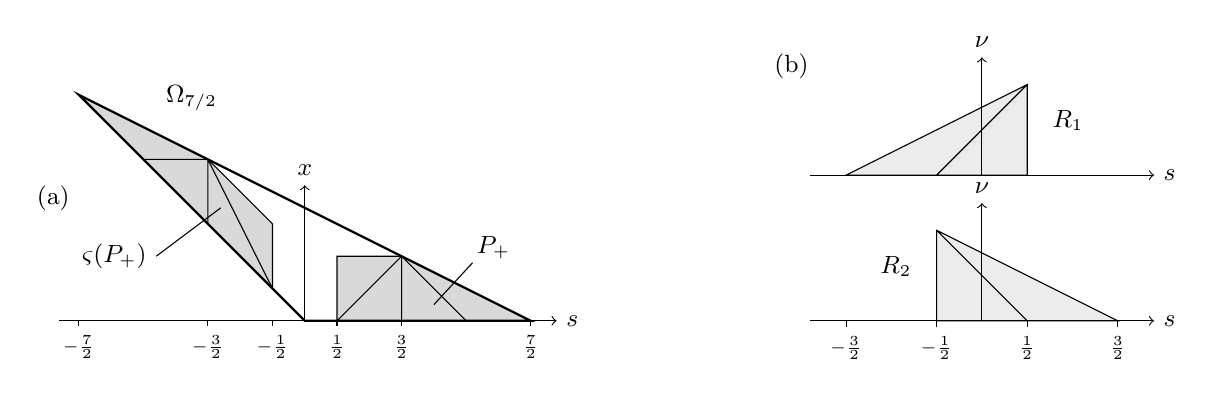
\begin{tikzpicture}[font=\small]
% ---- (a) the (s,x)-plane
\begin{scope}[x=0.82cm,y=0.82cm]
  \fill[gray!30] (0.5,0)--(3.5,0)--(1.5,1)--(0.5,1)--cycle;
  \fill[gray!30] (-0.5,0.5)--(-3.5,3.5)--(-1.5,2.5)--(-0.5,1.5)--cycle;
  \draw (0.5,0)--(1.5,1) (1.5,0)--(1.5,1) (2.5,0)--(1.5,1) (0.5,0)--(0.5,1)--(1.5,1);
  \draw (-0.5,0.5)--(-1.5,2.5) (-1.5,1.5)--(-1.5,2.5) (-2.5,2.5)--(-1.5,2.5) (-0.5,0.5)--(-0.5,1.5)--(-1.5,2.5);
  \draw[thick] (-3.5,3.5)--(0,0)--(3.5,0)--cycle;
  \draw[->] (-3.8,0)--(3.9,0) node[right]{$s$};
  \draw[->] (0,0)--(0,2.1) node[above]{$x$};
  \foreach \t/\l in {-3.5/-\frac72,-1.5/-\frac32,-0.5/-\frac12,0.5/\frac12,1.5/\frac32,3.5/\frac72}
    \draw (\t,0)--(\t,-0.08) node[below]{$\scriptstyle\l$};
  \draw (2.0,0.25)--(2.6,0.9) node[above right=-2pt]{$P_+$};
  \draw (-1.3,1.75)--(-2.3,1.0) node[left]{$\varsigma(P_+)$};
  \node[anchor=west] at (-4.3,1.9) {(a)};
  \node[anchor=west] at (-2.3,3.45) {$\Omega_{7/2}$};
\end{scope}
% ---- (b) the two columns in the (s,nu)-plane
\begin{scope}[xshift=8.6cm,yshift=1.85cm,x=1.15cm,y=1.15cm]
  \fill[gray!15] (-1.5,0)--(0.5,0)--(0.5,1)--cycle;
  \draw (-1.5,0)--(0.5,0)--(0.5,1)--cycle (-0.5,0)--(0.5,1);
  \draw[->] (-1.9,0)--(1.9,0) node[right]{$s$};
  \draw[->] (0,0)--(0,1.3) node[above]{$\nu$};
  \node at (0.95,0.6) {$R_1$};
  \node[anchor=west] at (-2.4,1.2) {(b)};
\end{scope}
\begin{scope}[xshift=8.6cm,yshift=0cm,x=1.15cm,y=1.15cm]
  \fill[gray!15] (-0.5,0)--(1.5,0)--(-0.5,1)--cycle;
  \draw (-0.5,0)--(1.5,0)--(-0.5,1)--cycle (0.5,0)--(-0.5,1);
  \draw[->] (-1.9,0)--(1.9,0) node[right]{$s$};
  \draw[->] (0,0)--(0,1.3) node[above]{$\nu$};
  \foreach \t/\l in {-1.5/-\frac32,-0.5/-\frac12,0.5/\frac12,1.5/\frac32}
    \draw (\t,0)--(\t,-0.07) node[below]{$\scriptstyle\l$};
  \node at (-0.95,0.6) {$R_2$};
\end{scope}
\end{tikzpicture}
\caption{Theorem~\ref{thm:family} for $n=3$: twelve balls in $B(\frac72)$. (a)~The region $\Omega_{7/2}$ in the
$(s,x)$-plane, the image of the moment triangle. The lower corner pieces $P_+$ and $\varsigma(P_+)$ (grey) are cut
into four unimodular triangles each; the white band above them is left for the columns. (b)~The two columns, in
the $(s,\nu)$-plane of the model, each cut into two unimodular triangles ($Q$ is empty since $h=1$). Over
$\frac12<s<\frac32$ the band has length $\frac12(\frac32-s)=u_{R_2}(s)$, symmetrically on the left, and over
$|s|<\frac12$ the columns have total height $\frac32$ while the band has length $c_A(s)$; the difference is the
profile of the concentric ball $B(\frac12)$.}
\label{fig:family}
\end{figure}

\begin{corollary}\label{cor:allk}
Let $k\ge3$ and $n=\lfloor\sqrt k\rfloor$. Put $A(k)=n$ if $k=n^2$, $A(k)=n+\frac12$ if $n^2<k\le n^2+n$, and
$A(k)=n+1$ otherwise. Then $k$ balls of capacity $1$ fit into $B(A(k))$, and
\[
\frac{k}{A(k)^2}\ \ge\ 1-\frac1{\sqrt k}.
\]
\end{corollary}

\begin{proof}
For $A=n$ or $n+1$ use the standard triangulation of $\Delta(A)$ into $A^2$ unimodular triangles (Traynor
\cite{Traynor1995}); for $A=n+\frac12$ use Theorem~\ref{thm:family} (here $n\ge2$, since $k\ge3$ and $k\le n^2+n$
exclude $n=1$), discarding surplus balls. For the inequality, $f(k)=k/A^2-1+k^{-1/2}$ has
$f'(k)=A^{-2}-\frac12k^{-3/2}>0$ for $n^2\le k$ and $A\le n+1$ when $n\ge2$, since $(n+1)^2<2n^3$; so on each range
of $k$ with fixed $A(k)$ it suffices to check the smallest $k$. For $k=n^2+1$, $A=n+\frac12$, the claim is
$(n-\frac34)\sqrt{n^2+1}\le n^2+n+\frac14$, which follows from $\sqrt{n^2+1}\le n+\frac1{2n}$. For $k=n^2+n+1$,
$A=n+1$, it is $n\sqrt{n^2+n+1}\le(n+1)^2$, which holds after squaring. The case $n=1$ is $k=3$, $A=2$.
\end{proof}

The constant is sharp for this family: $(1-k/A(k)^2)\sqrt k\to1$ along $k=n^2+1$.

\begin{proposition}\label{prop:ten}
There is a configuration in $B(\frac{19}6)$ with ten items. Hence ten balls of capacity $1$ fit into
$B(\frac{19}{6})$, with density $\frac{360}{361}$.
\end{proposition}

\begin{proof}
Let $A=\frac{19}6$. The upper corner items are the unimodular triangle $\Delta_X=\{(s,x)\in\Omega_A:s+x>A-1\}$
(that is, $\mu_1>A-1$), with $(s,x)$-vertices $(A-2,1),(A-1,0),(A,0)$, and its mirror $\Delta_Y=\varsigma(\Delta_X)$,
where $\varsigma(s,x)=(-s,s+x)$ is the swap $z_1\leftrightarrow z_2$. Then
$u^-=\beta$ and $u^+-u^-=\min\bigl(\frac12(A-|s|),\,A-1-|s|\bigr)$ for $|s|\le A-1$. There are eight
columns, each a single primitive-edge triangle $T(p,q)=\mathrm{conv}\{(p,0),(p+1,0),(q,1)\}$ with
\[
(p,q)\in\bigl\{(-\tfrac{13}6,-\tfrac76),(-\tfrac76,-\tfrac76),(-\tfrac76,-\tfrac12),(-\tfrac12,-\tfrac16),
(-\tfrac12,\tfrac16),(\tfrac16,\tfrac12),(\tfrac16,\tfrac76),(\tfrac76,\tfrac76)\bigr\}.
\]
The first two and last two are unimodular \emph{windows} ($q\in\{p,p+1\}$, so the triangle has a vertical
edge); the middle four are \emph{sheared windows} ($q-p\in\{\frac13,\frac23\}$), primitive-edge but not unimodular.
Figure~\ref{fig:ten} shows the profiles. Each profile $\ell_{T(p,q)}$ is the tent
vanishing at $p$ and $p+1$ with value $1$ at $q$, and $u_j=\ell_{T_j}$. The configuration is symmetric under
$s\mapsto-s$, and on $s\ge0$ the sum of the profiles is:
\[
\textstyle\sum_j\ell_{T_j}(s)=
\begin{cases}
\frac32,&0<s<\frac16,\\
\frac{19}{12}-\frac s2,&\frac16<s<\frac76\ \ (=c_A(s)),\\
\frac{13}6-s,&\frac76<s<\frac{13}6\ \ (=A-1-s),
\end{cases}
\]
and $0$ for $s>\frac{13}6$. For instance on $(\frac16,\frac12)$ the four items with nonzero profile are
$T(\frac16,\frac76)$, $T(\frac16,\frac12)$, $T(-\frac12,\frac16)$, $T(-\frac12,-\frac16)$, contributing
$(s-\frac16)+3(s-\frac16)+3(\frac12-s)+\frac32(\frac12-s)$, which equals $\frac{19}{12}-\frac s2$; the other intervals are checked in the same way. Since
$\frac32\le c_A(s)$ on $(0,\frac16)$, condition \eqref{eq:budget} holds. Theorem~\ref{thm:realise} gives the packing.
\end{proof}

Here too the free part of the bookkeeping is the profile $\max(0,\frac12(\frac16-|s|))$ of the concentric ball
$B(\frac16)$, of volume $\frac1{72}=\frac12(A^2-10)$. The four sheared items have apexes outside the coset of
their base points, so their profiles are not lattice profiles and Theorem~\ref{thm:tensor} below does not apply
to this configuration.

\begin{figure}[t]
\centering
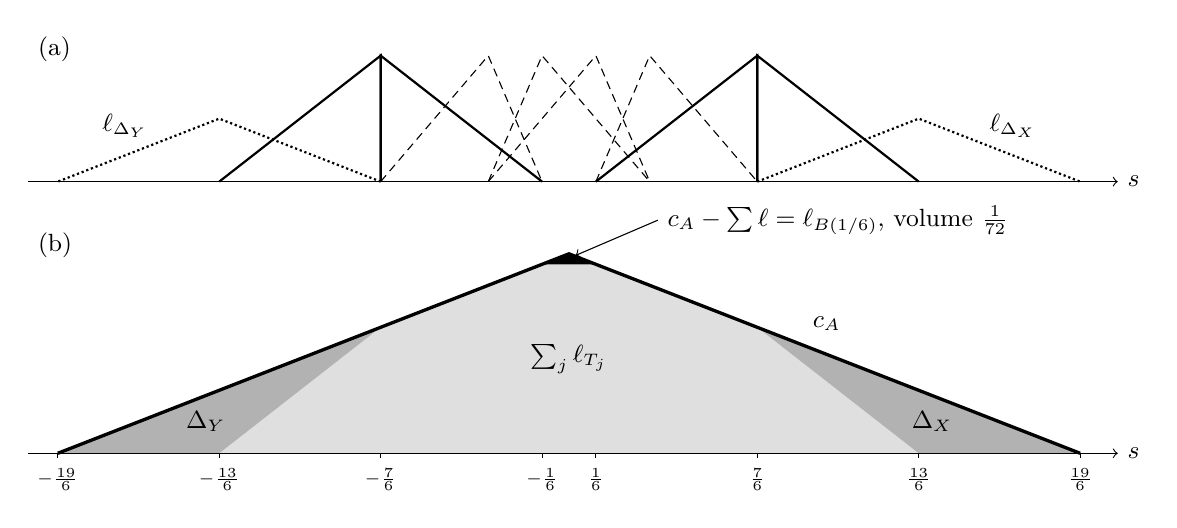
\begin{tikzpicture}[x=2.05cm,y=1.6cm,font=\small]
% ---- (a) individual profiles
\begin{scope}[yshift=3.45cm]
  \draw[->] (-3.35,0)--(3.4,0) node[right]{$s$};
  \foreach \p/\q/\r in {-2.16667/-1.16667/-1.16667,-1.16667/-1.16667/-0.16667,0.16667/1.16667/1.16667,1.16667/1.16667/2.16667}
    \draw[thick] (\p,0)--(\q,1)--(\r,0);
  \foreach \p/\q/\r in {-1.16667/-0.5/-0.16667,-0.5/-0.16667/0.5,-0.5/0.16667/0.5,0.16667/0.5/1.16667}
    \draw[densely dashed] (\p,0)--(\q,1)--(\r,0);
  \draw[densely dotted,thick] (1.16667,0)--(2.16667,0.5)--(3.16667,0);
  \draw[densely dotted,thick] (-1.16667,0)--(-2.16667,0.5)--(-3.16667,0);
  \node[anchor=west] at (-3.35,1.05) {(a)};
  \node[above] at (2.75,0.27) {$\ell_{\Delta_X}$};
  \node[above] at (-2.75,0.27) {$\ell_{\Delta_Y}$};
\end{scope}
% ---- (b) bookkeeping
\fill[gray!25] (-2.16667,0)--(-1.16667,1)--(-0.16667,1.5)--(0.16667,1.5)--(1.16667,1)--(2.16667,0)--cycle;
\fill[gray!60] (1.16667,1)--(3.16667,0)--(2.16667,0)--cycle;
\fill[gray!60] (-1.16667,1)--(-3.16667,0)--(-2.16667,0)--cycle;
\fill[black] (-0.16667,1.5)--(0,1.58333)--(0.16667,1.5)--cycle;
\draw[very thick] (-3.16667,0)--(0,1.58333)--(3.16667,0);
\draw[->] (-3.35,0)--(3.4,0) node[right]{$s$};
\foreach \t/\l in {-3.16667/-\frac{19}6,-2.16667/-\frac{13}6,-1.16667/-\frac76,-0.16667/-\frac16,0.16667/\frac16,1.16667/\frac76,2.16667/\frac{13}6,3.16667/\frac{19}6}
  \draw (\t,0)--(\t,-0.04) node[below]{$\scriptstyle\l$};
\node[anchor=west] at (-3.35,1.65) {(b)};
\node at (0,0.75) {$\sum_j\ell_{T_j}$};
\node at (2.25,0.25) {$\Delta_X$};
\node at (-2.25,0.25) {$\Delta_Y$};
\node[anchor=south west] at (1.45,0.9) {$c_A$};
\draw[<-] (0.04,1.57)--(0.55,1.85) node[right]{$c_A-\sum\ell=\ell_{B(1/6)}$, volume $\frac1{72}$};
\end{tikzpicture}
\caption{The ten-ball configuration of Proposition~\ref{prop:ten}, $A=\frac{19}6$. (a)~The profiles of the eight
column items: four windows (solid, with a vertical edge) and four sheared windows (dashed), each a tent of height
$1$ on an interval of length $1$; dotted, the profiles of the upper corner items $\Delta_X,\Delta_Y$. (b)~The
bookkeeping under the profile $c_A(s)=\frac12(A-|s|)$ of $B(A)$ (thick): the column profiles add up to the light
region, the corner items fill the dark triangles, and the only gap is the black triangle over $|s|<\frac16$,
the profile of the concentric ball $B(\frac16)$, of volume $\frac1{72}=\frac12(A^2-10)$.}
\label{fig:ten}
\end{figure}

% =====================================================================================================
\section{Obstructions}\label{sec:obstructions}

\subsection{The tensor area}\label{sec:tensor}
Regard $\R$ as a vector space over $\Q$ and let $\R\otimes\R=\R\otimes_\Q\R$. Let $\mathfrak M$ be the set of
distributions on $\R$ of the form
\[
m=\sum_v m_v\,\delta_v+\sum_w J_w\,\delta'_w\qquad(\text{finite sums},\ m_v\in\Q,\ J_w\in\R),
\]
with $\langle\delta'_w,f\rangle=-f'(w)$, and define
\[
\Dt(m)=\sum_v m_v\,v\otimes v-\sum_w\bigl(J_w\otimes w+w\otimes J_w\bigr)\ \in\R\otimes\R,
\]
the formal value of $m$ on $t\otimes t$. The multiplication map $\R\otimes\R\to\R$ sends $\Dt(m)$ to $\langle
m,t^2\rangle$.

\begin{lemma}\label{lem:D-translate}
If $\langle m,1\rangle=0$ and $\langle m,t\rangle=0$, then $\Dt$ of the translate of $m$ by any $\tau\in\R$ equals
$\Dt(m)$. This holds for $m=f''$ whenever $f$ is compactly supported and $f''\in\mathfrak M$.
\end{lemma}

\begin{proof}
The translate has $\Dt=\Dt(m)+M_1\otimes\tau+\tau\otimes M_1+M_0\,\tau\otimes\tau$ with $M_0=\sum m_v=\langle m,1\rangle\in\Q$ and
$M_1=\sum m_vv-\sum J_w=\langle m,t\rangle\in\R$. For compactly supported $f$, $\langle f'',1\rangle=\langle
f'',t\rangle=0$.
\end{proof}

A \emph{unit lattice profile} is a compactly supported piecewise linear function $\ell\ge0$ with $\int\ell=\frac12$
whose second derivative lies in $\mathfrak M$, has rational coefficients $J_w$, and is supported in one coset
$t+\Z$. The profile $\ell_T$ of a unimodular triangle $T$ is one: its breakpoints are the first coordinates of the
vertices, which lie in one coset of $\Z$; its slopes are rational; and a vertical edge, if any, has length $1$.

\begin{lemma}\label{lem:D-unit}
For a unit lattice profile $\ell$, $\Dt(\ell'')=1\otimes1$.
\end{lemma}

\begin{proof}
By Lemma~\ref{lem:D-translate} we may translate so that $t=0$. Then all points are integers and all coefficients
rational, so $\Dt(\ell'')=(\sum m_vv^2-2\sum J_ww)\,1\otimes1=\langle\ell'',t^2\rangle\,1\otimes1=2\int\ell\cdot1\otimes1$.
\end{proof}

A \emph{linear circle} is $S_f$, $f\in\Z^2$ primitive, with moment map $f\cdot\mu$. Complete $f$ to a matrix $M$
with rows $f,g$ and $\det M=1$. For a compact polygon $P\subset\R^2$ the \emph{$f$-profile} $c_{P,f}(u)$ is the
length of $\{y:(u,y)\in MP\}$; it does not depend on $g$, it is the density of the push-forward of Lebesgue measure on
$P$ under $f$, and $c_{\Delta(A),(1,-1)}=c_A$. The polygon is \emph{integral-directional} if each edge is parallel
to a vector of $\Z^2$. Then $c_{P,f}$ is piecewise linear, its slopes are rational because they are differences of
slopes of integer directions, and its jumps occur at edges with $f\cdot e=0$; so $c_{P,f}''\in\mathfrak M$.

\begin{lemma}\label{lem:tensor-area}
For an integral-directional polygon $P$, $\Dt(c''_{P,f})$ does not depend on $f$. Writing it as $2\,\area^\otimes(P)$,
$\area^\otimes$ is additive under subdivision into integral-directional polygons, and
\begin{enumerate}[label=(\alph*),leftmargin=2em]
\item $\area^\otimes(\lambda T_0+v)=\area(T_0)\,\lambda\otimes\lambda$ for a triangle $T_0$ with integer vertices and
  $\lambda>0$;
\item $\area^\otimes(P)=\frac12|\det(u_1,u_2)|\,(\lambda_1\otimes\lambda_2+\lambda_2\otimes\lambda_1)$ for the
  parallelogram $P=\{a+x\lambda_1u_1+y\lambda_2u_2:x,y\in[0,1]\}$, $u_i\in\Z^2$, $\lambda_i>0$.
\end{enumerate}
In particular $\area^\otimes(\Delta(A))=\frac12A\otimes A$.
\end{lemma}

\begin{proof}
For fixed $f$, profiles of polygons with disjoint interiors add, and $\Dt$ is additive on $\mathfrak M$; so
$P\mapsto\Dt(c''_{P,f})$ is additive. It therefore suffices to compute (a) and (b) and to show that every
integral-directional polygon is a union, with disjoint interiors, of integral-directional triangles and
parallelograms. For the last point, cut $P$ by the lines through its vertices in an integer direction $e$ not
parallel to any edge; the pieces are trapezoids with two sides parallel to $e$ and two sides along edges of $P$, and
a line through a vertex parallel to one of the latter splits each trapezoid into a parallelogram and a triangle,
both integral-directional. An integral-directional triangle has the form $\lambda T_0+v$ with $T_0$ integral: if
$d_1,d_2,d_3\in\Z^2$ are its edge directions, the edge lengths $(a,b,c)$ solve $ad_1+bd_2+cd_3=0$, an integer linear
system with one-dimensional solution space, so $(a,b,c)$ is a real multiple of an integer vector.

(a) Translation does not change $\Dt$ (Lemma~\ref{lem:D-translate}). The profile of $\lambda T_0$ is
$u\mapsto\lambda\,c_{T_0,f}(u/\lambda)$, whose second derivative has the same point masses at the points scaled by
$\lambda$ and jumps multiplied by $\lambda$. Since $c''_{T_0,f}$ has integer points and rational coefficients,
$\Dt=\langle c''_{T_0,f},t^2\rangle\,\lambda\otimes\lambda=2\area(T_0)\,\lambda\otimes\lambda$.

(b) Let $\alpha=\lambda_1f\cdot u_1$, $\beta=\lambda_2f\cdot u_2$. If both are nonzero, the profile is
$K\cdot\mathbf 1_{I_1}*\mathbf 1_{I_2}$ (up to translation), where $I_1,I_2$ are the intervals between $0$ and
$\alpha$, $\beta$ and $K=|\det(u_1,u_2)|/|f\cdot u_1\,f\cdot u_2|\in\Q$. Its second derivative is
$\pm K(\delta_0-\delta_\alpha-\delta_\beta+\delta_{\alpha+\beta})$, the sign being that of $\alpha\beta$, and
$\Dt=\pm K(\alpha\otimes\beta+\beta\otimes\alpha)=|\det(u_1,u_2)|(\lambda_1\otimes\lambda_2+\lambda_2\otimes\lambda_1)$.
If $f\cdot u_1=0$, the profile is $J\,\mathbf 1_{[w_0,w_1]}$ with $J=\lambda_1|\det(u_1,u_2)|/|f\cdot u_2|$ and
$w_1-w_0=\lambda_2|f\cdot u_2|$; its second derivative is $J\delta'_{w_0}-J\delta'_{w_1}$, and
$\Dt=J\otimes(w_1-w_0)+(w_1-w_0)\otimes J$, the same value. Finally $\Delta(A)=A\,\Delta(1)$ with $\area\Delta(1)=\frac12$.
\end{proof}

\begin{theorem}[Tensor area]\label{thm:tensor}
Let $\Delta(A)=P_1\cup\dots\cup P_r$ with integral-directional polygons $P_\rho$ with disjoint interiors, let
$f_1,\dots,f_r$ be primitive, and suppose that for each $\rho$
\[
c_{P_\rho,f_\rho}=\sum_{i\in I_\rho}\ell_i\quad\text{almost everywhere},
\]
where each $\ell_i$ is a unit lattice profile. Then $k=\sum_\rho|I_\rho|$ satisfies $k=A^2$, and $A$ is an
integer.
\end{theorem}

\begin{proof}
Taking second derivatives and applying Lemmas~\ref{lem:D-unit} and~\ref{lem:tensor-area},
\[
k\,1\otimes1=\sum_\rho\Dt(c''_{P_\rho,f_\rho})=\sum_\rho2\area^\otimes(P_\rho)=2\area^\otimes(\Delta(A))=A\otimes A .
\]
If $A\notin\Q$, choose a $\Q$-linear map $L:\R\to\Q$ with $L(1)=0$ and $L(A)=1$; applying $L\otimes L$ gives $0=1$.
So $A\in\Q$, and $A^2=k$ by multiplication; a rational square root of an integer is an integer.
\end{proof}

In the setting of Section~\ref{sec:setup}, a lattice configuration has unit lattice profiles, and it is exact
precisely when $\sum_T\ell_T=c_A$ almost everywhere (by \eqref{eq:bookkeeping}). Theorem~\ref{thm:tensor} with one
piece and $f=(1,-1)$ therefore says that exact lattice configurations exist only for square $k$; the same holds for
any other linear circle, and for configurations in which different integral-directional pieces of $\Delta(A)$ use
different circles. The invariant is genuinely two-dimensional: the number $\langle c'',t^2\rangle$ only sees the
volume, while its lift to $\R\otimes\R$ sees the irrationality of $\sqrt k$.

\begin{corollary}\label{cor:gap}
For every non-square $k$ there is $A_{\rm lat}(k)>\sqrt k$ such that every lattice configuration with $k$ items in $B(A)$ has
$A\ge A_{\rm lat}(k)$. Hence such configurations have density at most $\rho_k=k/A_{\rm lat}(k)^2<1$.
\end{corollary}

\begin{proof}
Let $A_{\rm lat}(k)$ be the infimum of $A$ for which there are unimodular triangles $T_1,\dots,T_k$ with
$\sum\ell_{T_i}\le c_A$ almost everywhere; by \eqref{eq:bookkeeping} every lattice configuration is admissible. The
profile of a unimodular triangle is the tent with base points $u_1<u_3$, apex $u_2\in[u_1,u_3]$, $u_2-u_1$ and
$u_3-u_1$ integers, and height $1/(u_3-u_1)$. Under $\sum\ell_{T_i}\le c_A$ the supports lie in $[-A,A]$, so for
bounded $A$ there are finitely many shapes and the translations range over a compact set. Profiles depend
continuously on the translation in $L^1$, and the constraint passes to $L^1$-limits since $c_{A_n}\to c_A$ uniformly.
So the infimum is attained, and at $A=\sqrt k$ the constraint would force equality almost everywhere, which
Theorem~\ref{thm:tensor} excludes.
\end{proof}

\subsection{The Newton barrier}\label{sec:newton}
For an integrable function $\ell$ with compact support let $P[\ell](x)=\sum_{j\in\Z}\ell(x+j)$ be its
$1$-periodisation, a function on $\T=\R/\Z$ with the same integral. For $0\le\alpha\le\frac12$ let
$h_\alpha(x)=\max(0,\frac12(\alpha-|x|))$ on $\T$, where $|x|$ is the distance to $0$; it is the profile of the
concentric ball $B(\alpha)$, periodised.

\begin{lemma}\label{lem:periodise}
Let $\alpha=\dist(A,\Z)$. Then $P[c_A]=\frac12(A^2-\alpha^2)+h_\alpha$ on $\T$.
\end{lemma}

\begin{proof}
$c_A''=\frac12\delta_{-A}-\delta_0+\frac12\delta_A$, so $P[c_A]''=\frac12\delta_{[A]}+\frac12\delta_{[-A]}-\delta_0$,
and $\{[A],[-A]\}=\{\alpha,-\alpha\}$ in $\T$. This is also $h_\alpha''$. A continuous function on $\T$ with vanishing
second derivative is constant, and the constant follows from $\int c_A=\frac{A^2}2$ and $\int h_\alpha=\frac{\alpha^2}2$.
\end{proof}

Call nonnegative integrable functions $\ell_1,\dots,\ell_k$ \emph{balanced} if $\sum_iP[\ell_i]$ is constant almost
everywhere on $\T$.

\begin{theorem}[Newton barrier]\label{thm:newton}
Let $\ell_1,\dots,\ell_k\ge0$ be balanced, $\int\ell_i=\frac12$, and $\sum_i\ell_i\le c_A$ almost everywhere. Then
\[
k\le A^2-\dist(A,\Z)^2,\qquad\text{equivalently}\qquad A\ge N(k)=\tfrac12\bigl(m+\tfrac km\bigr),
\]
where $m$ is the integer with $m^2-m<k\le m^2+m$. This applies to any packing of $B(A)$ by disjoint measurable sets
$X_i$ of volume $\frac12$, with $\ell_i$ the density of the push-forward of $\vol|_{X_i}$ under $s=\mu_1-\mu_2$.
\end{theorem}

\begin{proof}
Periodising $\sum\ell_i\le c_A$ gives $\frac k2=\sum P[\ell_i]\le\frac12(A^2-\alpha^2)+h_\alpha$ almost everywhere by
Lemma~\ref{lem:periodise}; the right side is continuous, so the inequality holds at $x=\frac12$, where
$h_\alpha=0$. For the equivalence, $\phi(A)=A^2-\dist(A,\Z)^2$ equals $2mA-m^2$ on $[m-\frac12,m+\frac12]$, is
continuous and increasing, and takes the values $m^2-m$ and $m^2+m$ at the ends of this interval. For a packing by
measurable sets, $\vol|_{B(A)}$ has density $c_A$ in $s$ (the action-angle coordinates
$(s,x,\theta,\varphi)$ carry $\vol$ to $ds\,dx\,d\theta\,d\varphi$), so disjointness gives $\sum\ell_i\le c_A$.
\end{proof}

The barrier is a statement about a property of the bookkeeping, not about equivariance: it holds for all packings,
and the content lies in the hypothesis. Two sources of balance are relevant here.
\begin{enumerate}[label=(\alph*),leftmargin=2em]
\item If $\ell$ is a unit lattice profile without jumps, then $P[\ell]''=(\sum_vm_v)\delta_{[t]}=0$, so $P[\ell]$ is
  constant. Thus every lattice configuration whose items have no vertical edges is balanced and satisfies
  $A\ge N(k)$, a quantitative form of Corollary~\ref{cor:gap} for such configurations, since $N(k)>\sqrt k$ for
  non-square $k$.
\item If $c_A-\sum_i\ell_i$ equals the unperiodised profile $\max(0,\frac12(\alpha-|s|))$ of $B(\alpha)$, then
  $\sum P[\ell_i]=P[c_A]-h_\alpha$ is constant. This is the case for Theorem~\ref{thm:family} ($\alpha=\frac12$) and
  Proposition~\ref{prop:ten} ($\alpha=\frac16$).
\end{enumerate}
By (b), $N(n(n+1))=n+\frac12$ and $N(10)=\frac{19}6$ are attained: these configurations are optimal among balanced
ones, and their loss is a concentric ball of capacity $\dist(A,\Z)$ that balance does not allow to shrink.

\begin{remark}\label{rem:mp}
The barrier gives $N(6)=\frac52$, $N(7)=\frac83$, $N(8)=\frac{17}6$, which are the sharp capacities
$\sqrt{k/p_k}$ of McDuff and Polterovich \cite{McDuffPolterovich1994} ($p_6=\frac{24}{25}$, $p_7=\frac{63}{64}$,
$p_8=\frac{288}{289}$). In each case the inequality $2mA\ge k+m^2$ coincides, up to a positive factor, with the
obstruction $dA\ge\sum a_i$ from an exceptional class $dL-\sum a_iE_i$: $2L-E_1-\dots-E_5$, $3L-2E_1-E_2-\dots-E_7$
and $6L-3E_1-2E_2-\dots-2E_8$ (for $k=6,7$ after division by $2$). For $k\ge10$, Biran's theorem
\cite{Biran1997} gives packings of density arbitrarily close to $1$, so for non-square $k\ge10$ the barrier is not
an obstruction to packing and reflects only the balance hypothesis; for $k=10$ it reads $6A\ge19$, while
$\sqrt{10}<\frac{19}6$.
\end{remark}

\subsection{Full-height single-ball columns}\label{sec:eight}
Let $a:[0,1]\to\R$ be non-decreasing and $1$-Lipschitz and put $b(\nu)=a(\nu)+1-\nu$, so that $b$ is non-increasing.
The function
\[
\ell(s)=\bigl|\{\nu\in[0,1]:a(\nu)<s<b(\nu)\}\bigr|
\]
is a \emph{full-height column profile}, with base $p=a(0)$ and apex $q=a(1)=b(1)$. The region
$\{(s,\nu):a(\nu)<s<b(\nu)\}$ has disc slices, area $\frac12$, support $(p,p+1)$ and height $1$. For linear $a$ it is
the primitive-edge triangle $T(p,q)$ with $p\le q\le p+1$; this includes the windows $q\in\{p,p+1\}$ and the sheared items of
Proposition~\ref{prop:ten}. Corner items may or may not have such profiles: the corner triangle with
$(s,x)$-vertices $(0,0),(1,0),(0,1)$ has profile $1-s$ on $(0,1)$, which is one, while the corner simplices
$\Delta_X,\Delta_Y$ of Proposition~\ref{prop:ten} have profiles of height $\frac12$.

The one-sided limits $\ell(s^-)=|\{a<s\le b\}|$ and $\ell(s^+)=|\{a\le s<b\}|$ exist by dominated convergence, and
if $\sum_i\ell_i\le c_A$ almost everywhere then $\sum_i\ell_i(s^\pm)\le c_A(s)$ for every $s$ and each choice of
side (the same side for all $i$), because $c_A$ is continuous.

\begin{lemma}\label{lem:apex}
$\ell(q^-)=1$ or $\ell(q^+)=1$.
\end{lemma}

\begin{proof}
Since $a\le q\le b$, $\ell(q^-)=1-|\{a=q\}|$ and $\ell(q^+)=1-|\{b=q\}|$. Both sets are intervals ending at $1$. If
both had positive length, at the larger of their left ends $\nu_0<1$ we would have $a(\nu_0)=b(\nu_0)$, contradicting
$b-a=1-\nu_0>0$.
\end{proof}

\begin{lemma}\label{lem:twopoint}
Let $x\le q\le y$ and $\vartheta=1-(y-x)$. For sides $\sigma,\tau\in\{-,+\}$ with $\sigma=-$ if $x=q$ and $\tau=+$
if $y=q$, we have $\ell(x^\sigma)+\ell(y^\tau)\ge\vartheta$.
\end{lemma}

\begin{proof}
Assume $\vartheta>0$. For $\nu<\vartheta$ the interval $[a(\nu),b(\nu)]$ contains $q$ and has length
$1-\nu>y-x$, so $a(\nu)<x$ or $b(\nu)>y$. The sets $\{\nu<\vartheta:a(\nu)<x\}$ and $\{\nu<\vartheta:b(\nu)>y\}$ are
initial segments of $[0,\vartheta)$ with union $[0,\vartheta)$, so one of them is all of $[0,\vartheta)$. In the
first case these $\nu$ satisfy $a(\nu)<x\le b(\nu)$, which counts them in $\ell(x^-)$, and if $x<q$ also
$a(\nu)\le x<b(\nu)$, which counts them in $\ell(x^+)$. The second case is symmetric.
\end{proof}

The pointwise inequality $\ell(x)+\ell(y)\ge1-(y-x)$ is false when $x=q$ or $y=q$ (a window at its vertical edge
has value $0$ there); only the one-sided form is used.

\begin{theorem}\label{thm:eight}
Let $\ell_1,\dots,\ell_n$, $n\ge8$, be full-height column profiles with $\sum_i\ell_i\le c_A$ almost everywhere.
Then $A\ge\frac{19}6$.
\end{theorem}

Nothing is assumed about the rest of $B(A)$: the other balls of a packing may be corner simplices, windows for
another circle, or anything else. The theorem applies to packings in which eight balls are carried by pairwise
disjoint $S$-invariant sets with full-height column profiles; disjointness is required of these carriers, not
only of the balls. By Proposition~\ref{prop:ten} the bound is attained, so in any such arrangement in $B(A)$ with
$A<\frac{19}6$ at most seven balls are carried by full-height columns.

\begin{proof}
If $A\ge4$ there is nothing to prove, so let $A<4$; then $c_A<2$. By Lemma~\ref{lem:apex} each profile has a side
$\sigma_i$ at its apex $q_i$ with $\ell_i(q_i^{\sigma_i})=1$; take $\sigma_i=-$ when both sides qualify. At any
point at most one profile has left limit $1$ and at most one has right limit $1$, since otherwise a one-sided sum
would reach $2>c_A$. Consequently at most two profiles share an apex, and if two do, one has $\sigma=-$ and only
its left limit equals $1$, the other has $\sigma=+$. Order the profiles so that $q_1\le\dots\le q_n$, with the
$\sigma=-$ profile first at a shared apex. Put $\nu_{ij}=\ell_j(q_i^{\sigma_i})$ and $V_i=\sum_{j\ne i}\nu_{ij}$.

\emph{Apex inequalities.} At $q_i$ on side $\sigma_i$: $1+V_i\le c_A(q_i)$. In particular $c_A(q_i)\ge1$, so
$|q_i|\le A-2$ and $\frac12(A-|q_i|)\le A-1-|q_i|$. Write $\bar\imath=n+1-i$ for the indices counted from the end
($\bar1=n$, $\bar2=n-1$, $\bar3=n-2$). We use
\[
1+V_1\le A-1+q_1,\quad 1+V_3\le\tfrac12(A+q_3),\quad 1+V_{\bar3}\le\tfrac12(A-q_{\bar3}),\quad 1+V_{\bar1}\le A-1-q_{\bar1} .
\]
\emph{Two-point inequalities.} Choose indices $i<j$ with $3<i<j<\bar3$, which is possible as $n\ge8$.
Lemma~\ref{lem:twopoint} applies to profile $2$ at $q_1\le q_2\le q_3$ with sides $\sigma_1,\sigma_3$: if
$q_1=q_2$ then $\sigma_1=-$, and if $q_2=q_3$ then $\sigma_3=+$ (three profiles cannot share an apex). In the same
way it applies to profiles $i$ and $j$ at $q_3\le q_i,q_j\le q_{\bar3}$ and to profile $\bar2$ at
$q_{\bar3}\le q_{\bar2}\le q_{\bar1}$. With $\vartheta=1-(q_{\bar3}-q_3)$ and $\max(0,\vartheta)\ge\frac12\vartheta$:
\[
\nu_{12}+\nu_{32}\ge1-(q_3-q_1),\quad \nu_{3i}+\nu_{\bar3i}\ge\vartheta,\quad
\nu_{3j}+\nu_{\bar3j}\ge\tfrac12\vartheta,\quad \nu_{\bar3\bar2}+\nu_{\bar1\bar2}\ge1-(q_{\bar1}-q_{\bar3}).
\]
The eight terms on the left are distinct summands of $V_1,V_3,V_{\bar3},V_{\bar1}$, and all summands are
nonnegative, so
\[
V_1+V_3+V_{\bar3}+V_{\bar1}\ge\tfrac72+q_1+\tfrac12q_3-\tfrac12q_{\bar3}-q_{\bar1}.
\]
Adding the four apex inequalities gives $4+V_1+V_3+V_{\bar3}+V_{\bar1}\le3A-2+q_1+\frac12q_3-\frac12q_{\bar3}-q_{\bar1}$.
The positions cancel and $\frac{15}2\le3A-2$, that is $A\ge\frac{19}6$.
\end{proof}

In Proposition~\ref{prop:ten} the eight column items, in the order of their apexes, give equality in all eight
inequalities used.

% =====================================================================================================
\section{Remarks and open questions}\label{sec:remarks}

Computer searches over configurations with small denominators find better configurations than
Corollary~\ref{cor:allk} for many $k$ and suggest that the loss $\frac12(A^2-k)$ can be kept bounded, which would
give density $1-O(1/k)$; we have no proof. For fixed non-square $k$, density tending to $1$ within
Definition~\ref{def:config} would require configurations that are neither lattice configurations nor balanced
(Corollary~\ref{cor:gap}, Theorem~\ref{thm:newton}), and for $k=10$ below $A=\frac{19}6$ at least three items
without full-height column profile (Theorem~\ref{thm:eight}); we do not know whether such configurations exist.

\begin{remark}[Numerical implementations]\label{rem:program}
The release of this paper includes two programs in \texttt{program/}. The first, \texttt{solution\_epoch.py}, outputs
Hamiltonians in the format of the Epoch AI problem \cite{Epoch} using lattice layouts found by computer search, windows
and sheared windows (for some $k$, e.g.\ $k=12$, not the best layout of Section~\ref{sec:families}): for square
$16\le k\le10^5$ it reaches $\eps\approx0.002$, for other $10<k\le10^5$ an explicit $\eps_{\min}(k)$, and for
$k=10$ it reaches $\eps=0.005$ with the configuration of Proposition~\ref{prop:ten}. Its correctness is supported by
numerical integration, not proved, and is not part of the theorems of this paper; the returned Hamiltonians have
exterior branch cuts away from the ball trajectories and, for $k=10$, a $C^2$ window seam. The second,
\texttt{solution\_embedding.py}, evaluates closed-form $C^4$ packing embeddings directly for every $k\ge10$
and $\eps\in(0,1)$, with complete proofs in the fourth paper of the release.
\end{remark}

\section*{Authorship and the role of AI}

Liang Song is the sole author and is responsible for the manuscript and its release. The mathematics and the text
were produced by AI systems, including GPT-6.1 Sol (OpenAI), Claude Opus 5.5 (Anthropic) and other models, working
in a research environment designed and directed by Liang Song, who chose the problem, assembled the literature and
context given to the systems, designed the verification pipeline and made the editorial decisions. The proofs in
this paper are not formalised; the finite identities in Section~\ref{sec:families} were also checked in exact
rational arithmetic.

\bibliographystyle{amsalpha}
\bibliography{refs}

\end{document}
